%!TEX root = project.tex

\chapter{System Evaluation}
\section{Testing}
Throughout the development process the program was tested more and more as each new piece of the backend system was added. The game performed very well at each stage and there were no catastrophic failures encountered just minor tweaks here and there regarding scaling and audio.
\newline

In theory the system should be able to be retro fitted to be used to facilitate a number of different types of games. We did not have time to conduct a test of this nature but it is definitely something that will be explored during future development.
\newline

\section{Drawbacks and Limitations}
Testing proved difficult on a standard PC. Unity 3d is a large and powerful piece of software that requires a lot of resources to run. This resulted in slow performance when testing for some members of the team. When tested on a standard laptop we found the game was extremely taxing on the GPU, 86 - 95\% output at times.
\newline

As a result the game would work fine from the login process to the procedural track generation but would sometimes result in the game character not begin able to move forward. Alternatively when run on custom built gaming PCs, which two members of the group have, they experienced no problems at all.
\newline

We encountered same issue with the game character while filming the video demonstration for our project. While recording our video on a non gaming PC, while running Unity and screen o matic, the game character became unresponsive to any forward movement. Having the two pieces of software running simultaneously caused a huge drain on the resources of the standard graphics card on the PC. Once the recording software stopped the game character behaved as normal.
\newline

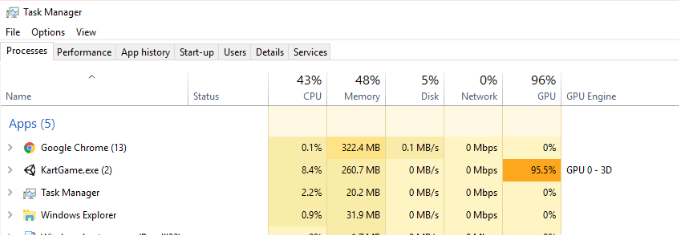
\includegraphics[width=1\columnwidth]{img/output.PNG}\newline
 
Another slight drawback was working with MongoDB as it was sometimes troublesome due to a lot of the java syntax for mongo being deprecated. A maven project approach might have been a better idea as there are more resources available with regards to working with mongo using java. 
\newline

The AWS virtual machine we used served its purpose as a free option but the initial set up, in terms of disc storage and RAM, was basic. We found out, throughout the development process, that we needed to restrict the amount of software installations on the VM. This was brought to our attention when the VMs performance had become extremely sluggish and sometimes unresponsive. 
\newline

As a result we decided to discuss any future software installations unless it was vital to the project. The removal of the eclipse IDE was a necessary step once the login process was up and running. This helped free up some space and memory for other resources that needed to be constantly active and running. In future, the implementation of a dedicated server to run the data bases might be a better option.
\newline

We originally intended to deploy the game on a mobile platform but unfortunately we did not have the time to achieve our goal. The games backend systems, match making and scoreboard system, were much larger tasks than originally thought so we decided to focus on  developing for VR and desktop only.

\section{Outcomes}
The project goals, as laid out in the introduction, was a success to a point. The processes involved in allowing a player to login works very well. The database and program running this process has been running since the start of the project and has never given us any difficulty since being implemented.
\newline

The hosting and joining system also works very well. The data that is required when sending and receiving to and from the databases does so very efficiently. And the list of hosts is updated and shown on screen.
\newline

The game works quite well. The procedural track is built very quickly and there is a different one built each time. All the players spawn at a different places on the start line, which was a problem at the beginning. The racers are all able to move left and right and the acceleration button works. The problem here was that on a non gaming laptop the player sometimes can not drive as the game is very taxing on some GPU's. The VR game also works well, both the VR and desktop players can see each other on the screen and can race against each other. We encountered a problem near the end though, the oculus was updated and the players hands were visible at a different position to the original placement.
\newline

Independently, the score board system works very well. A list of player objects is serialized into XML and is sent to the scores data base. The data base is updated and the players global position is updated and the new list is sent back. Results and leader board are then put on screen.
\newline

Unfortunately, we encountered a problem with the race results. The player object gets destroyed as they cross the finish line. The issue was there was not enough time to figure out how to structure the order in which they cross the line and send that information to the scoreboard. This was a big disappointment to us as we feel as though we have the ingredients for a really fun, exciting and fully functioning game.




